\documentclass[conference]{IEEEtran}
% ---------------------------------------------------------------------------
% Short Paper (IEEE conference format) --- Urban Mobility Equity Dashboard
% EMGT 7945 MS Project. Compile: tectonic Short_Paper.tex
% ---------------------------------------------------------------------------
\usepackage{cite}
\usepackage{microtype}
\usepackage{stfloats}
\usepackage{amsmath}
\usepackage{graphicx}
\usepackage{booktabs}
\usepackage{array}
\usepackage[hidelinks]{hyperref}
\graphicspath{{../data/outputs/figures/}}

\begin{document}

\title{A Reproducible Mobility Equity Score: Integrating Transit, Walkability,
Bicycle, and EV-Charging Supply at the Census-Tract Level}

\author{\IEEEauthorblockN{Aashritha Krishna Kanagala}
\IEEEauthorblockA{Master of Science in Engineering Management\\
Northeastern University, Boston, MA, USA\\
EMGT 7945 MS Project \quad Supervisor: Prof.\ Sivarit (Tony) Sultornsanee}}

\maketitle

\begin{abstract}
Urban mobility infrastructure---public transit, walkable streets, bicycle
facilities, and electric-vehicle (EV) charging---is unevenly distributed, yet
existing tools measure each dimension in isolation. We construct a
\emph{Mobility Equity Score} (MES): a transparent, reproducible composite index
that integrates all four dimensions at the U.S.\ Census-tract level, and apply
it to three structurally distinct cities (Chicago, Houston, Seattle) using only
open data. The MES is strongly spatially clustered in every city (global
Moran's $I=0.82$--$0.92$) and is positively associated with the share of
car-free and renter households. A bivariate negative association with median
income is shown to be largely a function of urban form: after controlling for
population density and distance to the central business district, and after
spatial-regression correction, it attenuates to non-significance in Houston,
reverses in Chicago, and persists only in Seattle. Findings are therefore
interpreted as associational and consistent with a supply--need mismatch. The
pipeline and an interactive dashboard are released open-source.
\end{abstract}

\begin{IEEEkeywords}
transportation equity, composite index, spatial analysis, GIS, open data,
mobility deserts
\end{IEEEkeywords}

\section{Introduction}
Access to jobs, health care, and education depends on a layered ecosystem of
transit, pedestrian, cycling, and---increasingly---EV-charging infrastructure,
each with documented equity gaps~\cite{aman2020,urban2022,lou2025,ahmed2024}.
Yet measurement remains siloed: the EPA walkability index, the DOE charger
locator, transit GTFS feeds, and OpenStreetMap bicycle data each capture one
dimension. No open, reproducible tool integrates all four into a single
neighborhood-level equity measure.

This paper contributes: (i) an open, reproducible integration of four mobility
dimensions into a tract-level composite; (ii) a transparent methodology whose
normalization, weighting, and thresholds are stress-tested; and (iii) an
empirical result---that the apparent income gradient in mobility supply is
largely an urban-form artifact---obtained through confounder controls and
spatial regression. The dashboard is a dissemination layer, not the
contribution.

\section{Related Work}
Single-dimension equity evidence is strong but isolated: transit
deserts~\cite{aman2020,maharjan2024}, racialized walkability~\cite{urban2022},
and severe EV-charging gaps for disadvantaged and renter
households~\cite{lou2025,chenli2024}. Composite-indicator methodology warns that
normalization and weighting are value-laden and require sensitivity
analysis~\cite{nardo2008}. Integrated tools exist but trade away tract-level,
multi-modal, or open-data properties (e.g., city-scale readiness indices, or
spending-based equity tools). The MES fills this gap and, unlike prior work,
\emph{measures} rather than assumes the direction of the supply--demographic
relationship.

\section{Methodology}
\subsection{Study Area and Data}
The unit of analysis is the 2023 Census tract for Cook County (Chicago; 1,332
tracts), Harris County (Houston; 1,115), and King County (Seattle; 495). All
inputs are open: GTFS (transit), the EPA Smart Location Database (walkability),
OpenStreetMap via OSMnx~\cite{boeing2017} (bicycle and EV charging points), the
Census ACS 5-year 2019--2023 (demographics), and TIGER/Line boundaries.

\subsection{Mobility Equity Score}
Each of four sub-indices (Table~\ref{tab:sub}) is min--max normalized to
0--100 \emph{within} each city, then combined as an equally weighted mean,
$\mathrm{MES}=\sum_k w_k\, s_k^{\text{norm}}$, $\sum_k w_k=1$. Because
normalization is within-city, cross-city \emph{levels} are not compared; only
patterns are. Tracts below the 25th MES percentile are mobility deserts; those
below the 25th percentile in $\geq 2$ sub-indices are compounded deserts.

\begin{table}[t]
\caption{The four MES sub-indices.}
\label{tab:sub}
\centering
\footnotesize
\begin{tabular}{@{}lll@{}}
\toprule
\textbf{Sub-index} & \textbf{Metric} & \textbf{Source} \\
\midrule
Transit & Stop density; AM-peak freq.; span & GTFS \\
Walkability & Nat.\ Walkability Index (areal) & EPA SLD \\
Bicycle & Bike-lane km/km$^2$ & OSM \\
EV charging & Charger count; dist.\ to DC-fast & OSM/AFDC \\
\bottomrule
\end{tabular}
\end{table}

\subsection{Analysis}
Pearson correlations (with Fisher-$z$ confidence intervals and a Spearman
robustness check) relate the MES to income, percent non-white, percent
zero-vehicle, and percent renter. Global and local Moran's $I$ (queen
contiguity, 999 permutations) test spatial clustering. K-means with
silhouette-selected $k$ and multi-seed Adjusted Rand Index (ARI) yields a stable
typology. Because the MES is spatially autocorrelated, we additionally fit
multivariable OLS with urban-form controls (population density, distance to the
central business district) and spatial-lag/error models, and we recompute the
MES without the EV layer as a robustness check.

\section{Results}
\subsection{Distribution and Equity Associations}
Walkability is the strongest dimension and dedicated cycling the weakest in all
cities. The MES is strongly spatially clustered (Table~\ref{tab:res}: Moran's
$I=0.82$--$0.92$, all $p<0.001$), so supply inequity is contiguous and
place-based. The MES is positively associated with car-free ($r=0.41$--$0.69$)
and renter ($r=0.53$--$0.69$) shares, and bivariately negatively with income
($r=-0.08$ to $-0.27$). Fig.~\ref{fig:map} maps the MES and its sub-indices.

\begin{table*}[t]
\caption{Per-city summary and robustness. Income associations attenuate under
urban-form controls and spatial regression (except Seattle); clusters are
perfectly stable (ARI); the EV layer is non-decisive.}
\label{tab:res}
\centering
\small
\begin{tabular}{@{}lcccccc@{}}
\toprule
\textbf{City} & \textbf{Tracts} & \textbf{Mean MES} & \textbf{Moran's $I$} & \textbf{MES--income (bivariate)} & \textbf{+ urban-form controls} & \textbf{Cluster ARI} \\
\midrule
Chicago & 1{,}332 & 37.5 & 0.92 & $-$ ($p{=}.002$) & $+$, weak & 1.00 \\
Houston & 1{,}115 & 31.7 & 0.83 & $-$ ($p{<}.001$) & n.s.\ ($p{=}.64$) & 1.00 \\
Seattle & 495 & 36.2 & 0.82 & $-$ ($p{<}.001$) & $-$ ($p{<}.001$) & 1.00 \\
\bottomrule
\end{tabular}
\end{table*}

\subsection{Confounding, Spatial Dependence, Robustness}
Adding density and CBD distance to an OLS of the MES on income changes the
income coefficient sharply: it becomes non-significant in Houston, reverses to
weakly positive in Chicago, and remains negative and significant only in
Seattle. Spatial-lag/error models (error preferred for Chicago, lag for Houston
and Seattle by AIC) corroborate this: once spatial dependence is modeled, the
income association is negligible except in Seattle. The K-means typology is
perfectly reproducible (mean ARI $=1.00$; silhouette $0.41$--$0.48$), and
dropping the OSM-sourced EV layer barely changes the income correlation
($|\Delta r|=0.002$--$0.053$). The desert classification is stable across the
20th/25th/30th percentiles (Jaccard $0.80$--$0.83$).

\begin{figure*}[b]
\centering
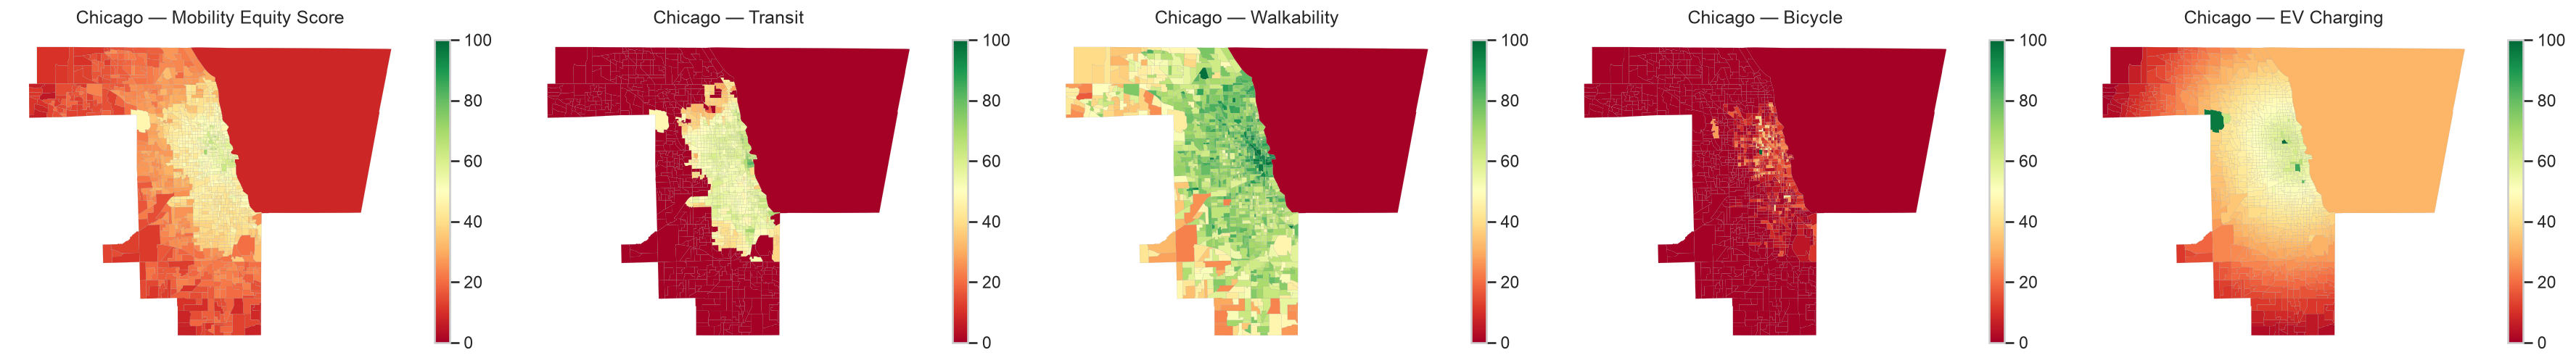
\includegraphics[width=\textwidth]{choropleth_chicago.png}
\caption{Chicago MES and its four sub-indices (green = better served, red =
worse). Walkability and transit concentrate centrally; dedicated bicycle
infrastructure is sparse citywide.}
\label{fig:map}
\end{figure*}

\section{Discussion and Conclusion}
\emph{What the data demonstrate:} mobility supply is strongly spatially
clustered, positively associated with car-free and renter shares, and its
apparent negative income gradient is largely an urban-form artifact that does
not survive density/centrality controls or spatial regression except in Seattle.
The composite is well-behaved---related-but-non-redundant sub-indices, stable
weighting, reproducible clusters, EV-insensitive conclusions.

\emph{What we infer:} because supply co-occurs with density (and thus with
car-free and renter populations), the equity question is best framed,
associationally, as a supply--\emph{need} mismatch; demand itself is not
modeled. Compounded deserts and low-low LISA cold spots locate the tracts where
car-free and minority households (52--64\% non-white in the Chicago/Houston
deserts) plausibly face the widest gap, and are where the framework adds most
policy value.

\emph{Limitations} are the supply-side scope, the OSM EV proxy, within-city
normalization (no cross-city levels), and a three-city cross-section. Future
work extends to more cities, substitutes authoritative AFDC EV and FTA transit
service-quality data, and adds demand-side accessibility. The full pipeline and
dashboard are open-source, making the method transferable to any city with open
data.

\begin{thebibliography}{00}
\bibitem{aman2020} J.~J. Aman and J.~Smith-Colin, ``Transit deserts: Equity analysis of public transit accessibility,'' \emph{J. Transp. Geogr.}, vol.~89, p.~102869, 2020.
\bibitem{urban2022} Urban Institute, ``Redefining Walkability: A Neighborhood-Level Analysis,'' Washington, DC, 2022.
\bibitem{lou2025} J.~Lou, A.~Chandra, and M.~Gordon, ``Equity and reliability of public EV charging stations in the United States,'' \emph{Nature Commun.}, vol.~16, p.~4201, 2025.
\bibitem{ahmed2024} S.~Ahmed, Z.~Sultana, and M.~Rahman, ``A systematic review of bicycle infrastructure design principles within urban bikeability indices,'' \emph{Sustainability}, vol.~17, no.~14, p.~6409, 2024.
\bibitem{maharjan2024} S.~Maharjan, F.~Janatabadi, and A.~Ermagun, ``Spatial inequity of transit and automobile access gap across America,'' \emph{Transp. Res. Rec.}, vol.~2678, no.~1, pp.~674--690, 2024.
\bibitem{chenli2024} X.~Chen and Y.~Li, ``Electric vehicle charging equity and accessibility: A U.S. policy analysis,'' \emph{Transp. Res. Part D}, vol.~118, p.~103748, 2024.
\bibitem{nardo2008} M.~Nardo \emph{et al.}, \emph{Handbook on Constructing Composite Indicators}. OECD/JRC, 2008.
\bibitem{boeing2017} G.~Boeing, ``OSMnx: New methods for acquiring, constructing, analyzing, and visualizing complex street networks,'' \emph{Comput. Environ. Urban Syst.}, vol.~65, pp.~126--139, 2017.
\end{thebibliography}

\end{document}
